% \blankpage
% \null
% \vfill
% \begin{center}
  \rmfamily
  % \fontspec{Gill Sans}
  \setstretch{1.0}

  %% TODO indiquer l'origine de la région convertie.
  %% TODO décaler les flèches bleues et rouge pour qu'elles correspondent mieux.

  \tikzset{trace text/.style = {align = left, below right, font = \scriptsize}}
  \tikzset{trace legend/.style = {Black, opacity = 1, align = center, text width = 4.5cm,
      above, font = \scriptsize}} %
  \tikzset{trace fleche/.style={Gray, dotted, thick, opacity = 0.6}}
  % \tikzset{trace text/.style={black, text width = 7cm, font = \scriptsize, above}}

  \begin{tikzpicture}

    %% Trace de conversion des donneurs strong

    \node[trace text] at (0, 0) {%
      \textcolor{white}{cuicui}\\ % un titre était présent ici. doublon avec le titre en bas. remplacé
         % par un blank space pour ne pas avoir à tout décaler.
      \includegraphics[width = 0.65\textwidth]{img/trace_ws.pdf}};

    \coordinate (complexe strong) at (8, -6.3);
    \coordinate (complexe weak) at (6.7, -6.3);
    \coordinate (badqual) at (1.4, -14);
    \coordinate (tout bleu) at (12, -13.5);

    % \draw[opacity = 0.2, line width = 0.01pt, Gray] (0,0) grid (15, -15);
    % \draw[opacity = 0.2, line width = 0.005pt, step = 0.5, Gray] (0,0) grid (15, -15);

    \draw[trace fleche, gs_rec_col] [<-] (10.2, -1.0) -- (12, -1.0)
    node[trace legend] {\textcolor{gs_rec_col}{Génotype du receveur}}
    node {\(\bullet\)}
    ;

    \draw[trace fleche, gs_don_col] [<-] (10.2, -14.35) -- (12, -14.35)
    node[trace legend] {\textcolor{gs_don_col}{Génotype du donneur}}
    node {\(\bullet\)}
    ;

    \draw[trace fleche] (11.5, -5) %
    node{\(\bullet\)} %
    node[trace legend, darkgray] {Restauration de l'haplotype sauvage GC.}
    -- ++(-1, 0) -- (complexe strong);

    \draw[trace fleche]  (11.5, -8) %
    node{\(\bullet\)} %
    node[trace legend, darkgray] {Restauration de l'haplotype sauvage AT.}
    -- ++(-1, 0) -- (complexe weak);

    %% flèche sens du séquençage
    \draw[trace fleche, opacity = 0.4] [->] (5, -0.3)
    node[left, font=\scriptsize, opacity = 0.5] {Sens du séquençage}
    % node{\(\bullet\)}
    -- ++(2, 0)
    ;

    % \draw[opacity = 0.2, line width = 0.01pt, Gray] (0,0) grid (15, -19);
    % \draw[opacity = 0.2, line width = 0.005pt, step = 0.5, Gray] (0, 0) grid (15, -19);
    % \draw[]

    \begin{scope}[shift={(-2, 11.0)}]

      \draw[gs_rec_col,    very thick] (5,    -10.0) -- (7, -10.0);
      \draw[ancre_don_col, very thick] (11.4, -10.0) -- ++(-0.5, 0);
      \draw[solid,         am1_col,           very thick] (7.0, -10.0) -- ++(0.2, 0);
      \draw[solid,         kanr_col,          very thick] (7.2, -10.0) -- ++(2.0, 0);
      \draw[solid,         genome_col,        very thick] (9.2, -10.0) -- ++(0.2, 0);
      \draw[solid,         ancre_don_col,     very thick] (9.4, -10.0) -- ++(1.5, 0);
      \draw[genome_col,    thick, arrows = {-Stealth[left]}] (11.4, -10.0) -- ++(1,   0);
      \draw[genome_col,    thick] (2, -10.0) -- (5, -10.0);

      %% brin <-
      \draw[gs_rec_col, very thick] (5, -10.2)   -- (5.5, -10.2);
      \draw[gs_don_col, solid,          very thick] (6.0, -10.2) -- ++(1.0,  0);
      \draw[gs_rec_col, solid,          very thick] (6.0, -10.2) -- ++(-0.5, 0);
      \draw[solid,      am1_col,        very thick] (7.0, -10.2) -- ++(0.2,  0);
      \draw[solid,      kanr_col,       very thick] (7.2, -10.2) -- ++(2.0,  0) node[midway, below, font = \tiny] {KanR};
      \draw[solid,      genome_col,     very thick] (9.2, -10.2) -- ++(0.2,  0);
      % \draw[solid,      ancre_don_col,  very thick] (9.4, -10.2) --   (9.9,  -10.2);
      \draw[solid,      ancre_don_col,  very thick] (9.4, -10.2) -- ++(2.0,  0) node[midway, below, font = \tiny] {Ancre};
      % génome
      \draw[genome_col, thick] (11.4, -10.2) -- ++(1, 0);
      \draw[genome_col, thick, arrows = {Stealth[left]-}] (2, -10.2) -- (5, -10.2);

	    \draw[Gray, thick, densely dotted, fill = Gray, opacity = 0.3] (6, -10.4) rectangle (7, -9.8);
      \node[Gray, font=\tiny] at (6.5, -10.55) {Hétéroduplex};

      \end{scope}

      \draw[dotted, Gray, line width = 1pt] (1 , -0.8) -- ++(2, +1.5);
      \draw[dotted, Gray, line width = 1pt] (10, -0.8) -- ++(-5, +1.5);

    % \node[trace legend, align = justify] at (13.5, -13) {%
    %   Chaque ligne horizontale représente une séquence. Les points représentent
    %   les positions des marqueurs sur les séquences. L'intensité et le diamètre
    %   des points représentent le score de qualité du site. La couleur des points
    %   représente leur polarité. Ils sont bleus lorsque le site est dans la
    %   région convertie : ils correspondent à l'haplotype du donneur. Ils sont
    %   rouges lorsque le site est dans la région conservée.

    %   Les alternances rouge / bleu marquent la transition de l'haplotype
    %   converti à l'haplotype sauvage : le point de recombinaison est localisé
    %   entre ces deux marqueurs.

    %   Les séquences sont triées par longueur de région convertie. Certains
    %   transformants ont converti tous les marqueurs\tikz[overlay]{\draw[gray,
    %     dotted, opacity = 0.9] [->] (0, 0) -- ++(-4, 10) -- ++(-1, 0);}.
    %   Certains transformants ont conservé tous les
    %   marqueurs\tikz[overlay]{\draw[gray, dotted, opacity = 0.7] [->] (0, 0) -- (-2, -1) -- (-3, -1);}.
    %   %
    % };
    %% DONE ajuster les flèches indiquant les séquences convertissant

  \end{tikzpicture}
\end{center}
% \caption[Zones de recombinaison détaillée]{\textbf{Zones de recombinaison entre
%     un locus génomique d'\emph{Acinetobacter baylyi} et un gène synthétique
%     donneur d'allèles GC et AT.} \\ %
%   \rmfamily Chaque ligne horizontale représente une séquence. Les points
%   représentent les positions des marqueurs sur les séquences. L'intensité et la
%   taille des points représentent le score de qualité de séquençage du site. Les
%   points sont bleus lorsque le site est dans la région convertie : ils
%   correspondent à l'haplotype du donneur. Ils sont rouges lorsque le site
%   correspond à l'haplotype du donneur. La première alternance rouge~/~bleu en
%   partant de l'extrémité 5' marque la transition de l'haplotype converti à
%   l'haplotype receveur : le point de recombinaison est localisé entre ces deux
%   marqueurs. Certaines séquences sont des cas de conversion complexes, avec une
%   ou plusieurs alternances donneur~/~receveur (rouge~/~bleu). Ce sont des cas de
%   conversion accompagnés de restaurations de l'haplotype du receveur. Les
%   séquences ont été triées par longueur de région convertie.}%
% \vfill
% \label{fig:convtract}
% \thispagestyle{empty}
% \addtocounter{page}{-1}
% % \afterpage{\blankpage}
% % \newpage
\

%% fréquences de transformation et distirbutino des points de bascule
\null
\vfill
\begin{table}[h!]
  \rmfamily
  \centering

  \caption[Fréquences de transformation]{\textbf{Fréquences de transformation
      chez \emph{A. baylyi}}}
  \label{tab:transfo-freq}
  \vspace{0.5cm}

  \begin{tabular}{cc}
    \toprule
    \thead{\normalsize Construction \\ \normalsize donneuse} & \thead{\normalsize Fréquences de \\ \normalsize transformation} \\
    \midrule
    GC    & \num{6.53e-5} \\
    AT    & \num{2.42e-5} \\
    AT/GC & \num{4.97e-5} \\
    GC/AT & \num{1.74e-4} \\
    \bottomrule
  \end{tabular}
\end{table}

\vfill

\begin{center}

  \begin{figure}

    \centering
    \tikzset{legende fleche/.style={Gray, dotted, thick, opacity = 0.6}}
    \rmfamily
    \scriptsize

    \begin{tikzpicture}[scale = 0.5]
      \node[above] at (0, 0) {\includegraphics[scale = 0.5]{img/pic_second.png}};
      % \draw[opacity = 0.2, line width = 1pt, Gray] (-15,0) grid (15, 15);
      % \draw[opacity = 0.2, line width = 0.005pt, step = 0.5, Gray] (-15,0) grid (15, +15);

      \draw[legende fleche] [->] (-6, 0)        node[ above] {Score de qualité} -- ++(4.5, 0) -- ++(1, 1);
      \draw[legende fleche, Black] [->] (-6, 7) node[ above] {Base G} -- ++(4.5, 0) -- ++(1, -1);
      \draw[legende fleche, Red3] [->] (-6, 11) node[ above] {Base T} -- ++(4.5, 0) -- ++(1, -1);

    \end{tikzpicture}

    \caption[Marqueur montrant des traces de contaminations]{%
      \textbf{Exemple de marqueur montrant des traces de
        contaminations} \\ \rmfamily Cet électrophérogramme montre les bases autour du
      marqueur à la position 200. Dans une région de qualité moyenne élevée (bases en
      5' et en 3'), le marqueur présente une trace de contamination par une autre
      base. La base déterminée est la base T mais une base G est présente dans la
      population d'amplicon séquencée.
      \label{fig:pic-second}
    }
  \end{figure}

  \begin{figure}[h!]

    \centering

    \tikzset{legende fleche/.style={Gray, thick}}
    \begin{tikzpicture}[scale = 0.3]
      \scriptsize
      \foreach \x in {1,2,...,12} {
        \foreach \y in {1,2,...,8} {
        \draw (\x, \y) circle (0.3cm) ;
      }}
    \draw[fill = Red] (8, 5) circle (0.3cm);
    \draw[fill = Red] (7, 6) circle (0.3cm);
    \draw[fill = Red] (7, 4) circle (0.3cm);
    \draw[fill = Red] (6, 5) circle (0.3cm);

    \draw[Gray, densely dotted] (5.5, 3.5) rectangle (8.5, 6.5);
    \draw[Gray, densely dotted] (9.5, 0.6) rectangle (12.4, 3.5);
    \draw[Gray] (0.5, 0.5) rectangle (12.5, 8.5);

    \draw[legende fleche] [<-] (7, 5) -- ++(1, 0.5) -- ++(5, 0)
    node[right, Black] {\(\bar{n} = \frac{4}{8} = \frac{1}{2}\)}
    ;

    \draw[legende fleche] [<-] (11, 2) -- ++(1, 2.0) -- ++(1, 0)
    node[right, Black] {\(\bar{n} = \frac{0}{8} = 0\)}
    ;

    \node[right] at (12.5, 8) {\(\bar{X} = 4\)};
    \node[right] at (12.5, 1) {\(\bar{N} = \sum_{i = 1}^{96}\frac{\bar{n_i}}{96}\)};

    \draw [->] (18.5, 4.5) -- ++(5, 0) node[midway, above] {\(\times 10000\)}
    node[right] {
      \includegraphics[width = 0.5\textwidth]{img/randomweak.png}
    };
    \end{tikzpicture}


    \caption[Des contaminations dues au hasard ?]{%
      \label{fig:simul-count}\textbf{Des contaminations dues au hasard ? } \\
      \rmfamily Par plaque de 96 puits, nous avons déterminé \(X\) le nombre de
      puits dont la séquence montre des traces de pics secondaires (voir
      figure~\ref{fig:pic-second}) et mesuré \(\bar{n}\) la moyenne du nombre de
      puits voisins contaminés. \(\bar{N}\) est la moyenne des 96 \(\bar{n}\)
      obtenus par plaque. Nous avons simulé \num{1e4} plaques avec \(X\) puits
      contaminés répartis aléatoirement, mesuré \(\bar{N}\) et comparé la valeur
      expérimentale de \(\bar{N}\) (trait vertical rouge) avec la distribution
      des \num{1e4} \(\bar{N}\) (en gris) Seules \(78 / 10000\) plaques simulées
      montrent un \(\bar{N}\) supérieur à la valeur expérimentale : la
      répartition des séquences contaminées dans les plaques ne peut pas être
      attribuée au hasard.
      %
    }
    % TODO légender figure pics secondaire simul
  \end{figure}

\end{center}

\vfill
\thispagestyle{empty}
\addtocounter{page}{-1}
\clearpage
\newpage


% ==============================================================================
\section{Résultats}
\label{sec:resultats}
% ==============================================================================

\afterpage{%
  \null
  \vfill


  \begin{center}
  \rmfamily
  % \fontspec{Gill Sans}
  \setstretch{1.0}

  %% TODO indiquer l'origine de la région convertie.
  %% TODO décaler les flèches bleues et rouge pour qu'elles correspondent mieux.

  \tikzset{trace text/.style = {align = left, below right, font = \scriptsize}}
  \tikzset{trace legend/.style = {Black, opacity = 1, align = center, text width = 4.5cm,
      above, font = \scriptsize}} %
  \tikzset{trace fleche/.style={Gray, dotted, thick, opacity = 0.6}}
  % \tikzset{trace text/.style={black, text width = 7cm, font = \scriptsize, above}}

  \begin{tikzpicture}

    %% Trace de conversion des donneurs strong

    \node[trace text] at (0, 0) {%
      \textcolor{white}{cuicui}\\ % un titre était présent ici. doublon avec le titre en bas. remplacé
         % par un blank space pour ne pas avoir à tout décaler.
      \includegraphics[width = 0.65\textwidth]{img/trace_ws.pdf}};

    \coordinate (complexe strong) at (8, -6.3);
    \coordinate (complexe weak) at (6.7, -6.3);
    \coordinate (badqual) at (1.4, -14);
    \coordinate (tout bleu) at (12, -13.5);

    % \draw[opacity = 0.2, line width = 0.01pt, Gray] (0,0) grid (15, -15);
    % \draw[opacity = 0.2, line width = 0.005pt, step = 0.5, Gray] (0,0) grid (15, -15);

    \draw[trace fleche, gs_rec_col] [<-] (10.2, -1.0) -- (12, -1.0)
    node[trace legend] {\textcolor{gs_rec_col}{Génotype du receveur}}
    node {\(\bullet\)}
    ;

    \draw[trace fleche, gs_don_col] [<-] (10.2, -14.35) -- (12, -14.35)
    node[trace legend] {\textcolor{gs_don_col}{Génotype du donneur}}
    node {\(\bullet\)}
    ;

    \draw[trace fleche] (11.5, -5) %
    node{\(\bullet\)} %
    node[trace legend, darkgray] {Restauration de l'haplotype sauvage GC.}
    -- ++(-1, 0) -- (complexe strong);

    \draw[trace fleche]  (11.5, -8) %
    node{\(\bullet\)} %
    node[trace legend, darkgray] {Restauration de l'haplotype sauvage AT.}
    -- ++(-1, 0) -- (complexe weak);

    %% flèche sens du séquençage
    \draw[trace fleche, opacity = 0.4] [->] (5, -0.3)
    node[left, font=\scriptsize, opacity = 0.5] {Sens du séquençage}
    % node{\(\bullet\)}
    -- ++(2, 0)
    ;

    % \draw[opacity = 0.2, line width = 0.01pt, Gray] (0,0) grid (15, -19);
    % \draw[opacity = 0.2, line width = 0.005pt, step = 0.5, Gray] (0, 0) grid (15, -19);
    % \draw[]

    \begin{scope}[shift={(-2, 11.0)}]

      \draw[gs_rec_col,    very thick] (5,    -10.0) -- (7, -10.0);
      \draw[ancre_don_col, very thick] (11.4, -10.0) -- ++(-0.5, 0);
      \draw[solid,         am1_col,           very thick] (7.0, -10.0) -- ++(0.2, 0);
      \draw[solid,         kanr_col,          very thick] (7.2, -10.0) -- ++(2.0, 0);
      \draw[solid,         genome_col,        very thick] (9.2, -10.0) -- ++(0.2, 0);
      \draw[solid,         ancre_don_col,     very thick] (9.4, -10.0) -- ++(1.5, 0);
      \draw[genome_col,    thick, arrows = {-Stealth[left]}] (11.4, -10.0) -- ++(1,   0);
      \draw[genome_col,    thick] (2, -10.0) -- (5, -10.0);

      %% brin <-
      \draw[gs_rec_col, very thick] (5, -10.2)   -- (5.5, -10.2);
      \draw[gs_don_col, solid,          very thick] (6.0, -10.2) -- ++(1.0,  0);
      \draw[gs_rec_col, solid,          very thick] (6.0, -10.2) -- ++(-0.5, 0);
      \draw[solid,      am1_col,        very thick] (7.0, -10.2) -- ++(0.2,  0);
      \draw[solid,      kanr_col,       very thick] (7.2, -10.2) -- ++(2.0,  0) node[midway, below, font = \tiny] {KanR};
      \draw[solid,      genome_col,     very thick] (9.2, -10.2) -- ++(0.2,  0);
      % \draw[solid,      ancre_don_col,  very thick] (9.4, -10.2) --   (9.9,  -10.2);
      \draw[solid,      ancre_don_col,  very thick] (9.4, -10.2) -- ++(2.0,  0) node[midway, below, font = \tiny] {Ancre};
      % génome
      \draw[genome_col, thick] (11.4, -10.2) -- ++(1, 0);
      \draw[genome_col, thick, arrows = {Stealth[left]-}] (2, -10.2) -- (5, -10.2);

	    \draw[Gray, thick, densely dotted, fill = Gray, opacity = 0.3] (6, -10.4) rectangle (7, -9.8);
      \node[Gray, font=\tiny] at (6.5, -10.55) {Hétéroduplex};

      \end{scope}

      \draw[dotted, Gray, line width = 1pt] (1 , -0.8) -- ++(2, +1.5);
      \draw[dotted, Gray, line width = 1pt] (10, -0.8) -- ++(-5, +1.5);

    % \node[trace legend, align = justify] at (13.5, -13) {%
    %   Chaque ligne horizontale représente une séquence. Les points représentent
    %   les positions des marqueurs sur les séquences. L'intensité et le diamètre
    %   des points représentent le score de qualité du site. La couleur des points
    %   représente leur polarité. Ils sont bleus lorsque le site est dans la
    %   région convertie : ils correspondent à l'haplotype du donneur. Ils sont
    %   rouges lorsque le site est dans la région conservée.

    %   Les alternances rouge / bleu marquent la transition de l'haplotype
    %   converti à l'haplotype sauvage : le point de recombinaison est localisé
    %   entre ces deux marqueurs.

    %   Les séquences sont triées par longueur de région convertie. Certains
    %   transformants ont converti tous les marqueurs\tikz[overlay]{\draw[gray,
    %     dotted, opacity = 0.9] [->] (0, 0) -- ++(-4, 10) -- ++(-1, 0);}.
    %   Certains transformants ont conservé tous les
    %   marqueurs\tikz[overlay]{\draw[gray, dotted, opacity = 0.7] [->] (0, 0) -- (-2, -1) -- (-3, -1);}.
    %   %
    % };
    %% DONE ajuster les flèches indiquant les séquences convertissant

  \end{tikzpicture}
\end{center}
  \caption[Zones de recombinaison détaillée]{\textbf{Zones de recombinaison entre
      un locus génomique d'\emph{Acinetobacter baylyi} et un gène synthétique
      donneur d'allèles GC et AT.} \\ %
    \rmfamily Chaque ligne horizontale représente une séquence. Les points
    représentent les positions des marqueurs sur les séquences. L'intensité et la
    taille des points représentent le score de qualité de séquençage du site. Les
    points sont bleus lorsque le site est dans la région convertie : ils
    correspondent à l'haplotype du donneur. Ils sont rouges lorsque le site
    correspond à l'haplotype du donneur. La première alternance rouge~/~bleu en
    partant de l'extrémité 5' marque la transition de l'haplotype converti à
    l'haplotype receveur : le point de recombinaison est localisé entre ces deux
    marqueurs. Certaines séquences sont des cas de conversion complexes, avec une
    ou plusieurs alternances donneur~/~receveur (rouge~/~bleu). Ce sont des cas de
    conversion accompagnés de restaurations de l'haplotype du receveur. Les
    séquences ont été triées par longueur de région convertie.}%
  \label{fig:convtract}
  \vfill
  \thispagestyle{empty}
  \addtocounter{page}{-1}
  \clearpage
  \newpage
}

\subsection{Validation de la démarche expérimentale}
\label{sub:result-proto}

Nous avons transformé une suspension d'\emph{Acinetobacter baylyi} par des
constructions dont l'intégration dans le génome par recombinaison homologue
entraîne la réparation des mésappariemments.

Les fréquences de transformations obtenues, représentées dans le tableau
\ref{tab:transfo-freq} sont de l'ordre de \num{1e-5} et ont permis d'obtenir un
grand nombre de recombinants, avec une moyenne de \num{9.2e+02} transformants
par boîte étalée, soit près de \num{3000} clones par transformation. Ce résultat
indique que le protocole expérimental est suffisamment au point pour permetter
d'obtenir le nombre de recombinants souhaité. Pour chaque gène de synthèse
donneur, \num{96} clones ont été séquencés, soit un total de \num{384}
recombinants.

\subsection{Validation de la qualité des séquences}
\label{sub:result-qualite}

Deux séquences trop courtes pour être alignées ont été exclues de l'analyse.
Neuf autres séquences présentaient une qualité médianne significativement
inférieure à celle des autres séquences et ont également été exclues. Au total,
\num{8561} marqueurs correspondant à des positions variantes entre le donneur et
le receveur ont été analysées. Globalement, la qualité des \num{373} séquences
suit un profil attendu : la qualité médianne est de \num{51} tout au long de la
séquence, à l'exclusion des bases situées aux extrémités 5' et 3'.

Cependant, \num{9.8}\% des marqueurs sont d'une qualité de séquençage inférieure
à la qualité de la région environnante. L'examen des électrophérogrammes a
révélé la présence de pics secondaires (voir figure~\ref{fig:pic-second}). Des
pics secondaires apparaissent quand la population d'amplicon séquencée n'est pas
homogène au site considéré. Or les deux pics présents à un marqueur donné
correspondent toujours soit à la base sauvage, soit à la base synthétique
introduite. Cette donnée peut être interprétée de deux façons.

1) Cette hétérogénéité pourrait résulter d'un signal biologique authentique : si
les mésappariemments de l'hétéroduplex ne sont pas réparés, la division de la
cellule mère conduirait à une colonie hétérogène au site considéré et donc à la
ségrégation simultanée des deux allèles. Pour tester cette hypothèse, nous avons
séquencé à nouveau \num{31} isolats issus d'un clone séquencé en premier lieu et
qui montrait des pics secondaires. Aucun des sous-clones séquencé ne montrent
l'allèle correspondant au pic secondaire (voir
figure~\ref{fig:confirm-haplotype}). Ceci indique que le clone initial n'était
pas hétérogène.

2) Une hypothèse alternative est que cette hétérogénéité pourrait être due à de
la contamination entre échantillons. Nous avons donc analysé la répartition dans
les plaques des puits dont la séquence montre des traces de contamination. Cette
analyse montre que les séquences présentant des pics secondaires sont plus
souvent voisines avec une autre séquence affectée que si elles étaient réparties
aléatoirement (voir figure~\ref{fig:simul-count}). Ce résultat indique que ces
pics secondaires correspondent très probablement à de la contamination. Pour
éviter les artéfacts liés à ces contaminants, nous avons décidé de n'étudier que
les marqueurs dont la qualité est supérieure à 40~: cela correspond à la
probabilité \num{1e-4} d'étudier une base déterminée à tort, et discrimine
clairement les bases litigieuses des autres. Nous avons donc obtenu un ensemble
de \num{6818} marqueurs de conversion, soit \SI{79.6}{\percent} de l'ensemble
des marqueurs obtenus.

\subsection{Description des régions recombinantes}
\label{subsec:result-descript}

\afterpage{%
  \null
  \vfill

  \begin{figure}
    \includegraphics[scale = 0.9]{img/distr_rcb_pt.pdf}
    \caption[Distribution de la position du dernier marqueur]{%
      \textbf{Distribution de la position du dernier marqueur converti} \\
      \rmfamily Ce graphique représente en ordonnées le nombre de transformants
      dont le dernier marqueur converti est à la position représentée en
      abscisse. Les panneaux du graphique représentent les quatres constructions
      donneuses. La position du dernier marqueur converti indique la position du
      point de recombinaison. Les transformants qui ne montrent aucun marqueur
      converti sont indiqués par des $N$.%
    }
    \label{fig:distrircb}
  \end{figure}
  \vfill

  \begin{table}[h!]
    \centering
    \rmfamily

    \caption[Dénombrement des cas de restauration]{\textbf{Dénombrement des cas de
        restauration} \\
      \rmfamily       %
    }
    \label{tab:restaur}

    \begin{tabular}{@{}ccc@{}}
      \toprule
      & \multicolumn{2}{c}{Nucléotide restauré} \\
      \cmidrule(r){2-3}
      \thead{\normalsize ADN synthétique \\ \normalsize donneur } & AT & GC \\
      \midrule
      AT    & - & 4 \\
      GC    & 0 & - \\
      AT/GC & 3 & 2 \\
      GC/AT & 1 & 4 \\
      \midrule[0.1pt]
      Total & 4 & 10 \\
      \bottomrule

    \end{tabular}
  \end{table}

  \vfill
  \thispagestyle{empty}
  \addtocounter{page}{-1}
  \clearpage
  \newpage
}

La figure \ref{fig:convtract} représente le détail des zones de recombinaison
obtenues avec une construction donneuse alternant GC et AT. Les zones de
recombinaisons des clones transformés par les donneurs GC, AT et AT/GC sont
détaillées en annexe \ref{subsec:trac-de-conv}. En moyenne, à notre locus cible,
\num{393} \(\pm\) \num{228} nucléotides ont été transférés et intégrés dans le
génome. La position du dernier marqueur converti indique le point de
recombinaison (voir figure~\ref{fig:recomb} et~\ref{fig:convtract}) qui se situe
entre les 30 bases le séparant du premier marqueur conservé. Nous avons donc
estimé la position du point de recombinaison par celle du dernier marqueur
converti, dont la distribution est représentée dans la
figure~\ref{fig:distrircb}. Les points de recombinaison se répartissent de façon
assez uniforme tout le long de la séquence. La majorité des recombinants
correspondent à des cas de conversion simple, avec une seule alternance entre
l'haplotype du donneur et celui du receveur. Cependant, \num{12} recombinants
montrent des cas de conversion complexes, avec au moins deux alternances entre
l'haplotype donneur et receveur. Ces alternances correspondent à des
restaurations de l'haplotype receveur dans l'hétéroduplex, qui peuvent résulter
de corrections ponctuelles des mésappariemments de l'hétéroduplex (voir
figure~\ref{fig:convtract}).

Nous nous sommes intéressés à deux paramètres permettant d'estimer les
fréquences de conversion en faveur de GC chez \emph{A. baylyi} : la position du
point de recombinaison, et la correction ponctuelle des mésappariemments.


% ------------------------------------------------------------------------------
\subsection{Comparaison de la longueur des régions converties}
\label{subsec:longueur}
% ------------------------------------------------------------------------------

La longueur moyenne de région convertie par les donneurs GC et AT est de
respectivement \num{446.6} et \num{395.6} pb ; l'écart entre les deux n'est pas
significatif (test de Wilcoxon, probabilité critique~\(=\) \num{0.31}) (voir
figure \ref{fig:distrircb}). De la même façon, la différence entre la longueur
de région convertie par le donneur dAT/GC et celle par le donneur dGC/AT n'est
pas significative (test de Wilcoxon, probabilité critique~\(=\)~\num{0.22}).
Globalement, le type de construction donneuse n'explique pas la variabilité de
la longueur de région convertie (test de Kruskal-Wallis, probabilité
critique~\(=\) \num{0.10}). Le type de donneur n'a pas d'influence sur la
longueur de région convertie.

% ------------------------------------------------------------------------------
\subsection{Restaurations de l'haplotype sauvage}
\label{subsec:restaur}
% ------------------------------------------------------------------------------

% tables de comptage des cas de restaurations
\afterpage{
  \null
  \vfill

  \begin{table}[h!]
    \centering
    \rmfamily
    \caption[Dénombrement des cas de conversion]{\textbf{Dénombrement des cas de conversion}}
    \label{tab:contingence}

    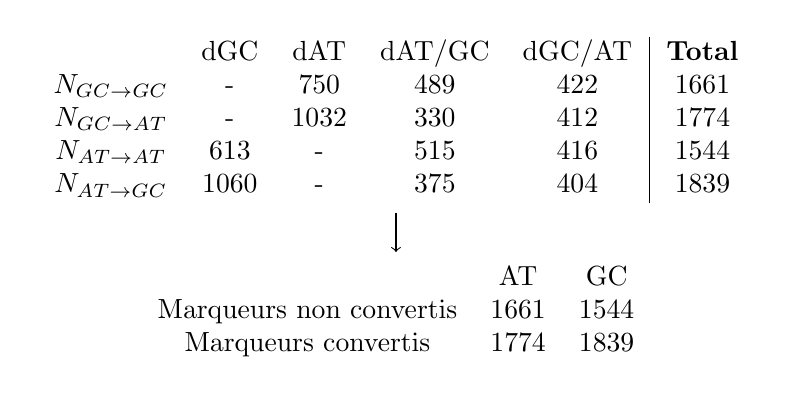
\begin{tikzpicture}[scale= 0.5]
      \draw [->] (0, 0) node[above]  {
        \begin{tabular}{ccccc|c}
          \toprule
                                  & dGC  & dAT  & dAT/GC & dGC/AT & \textbf{Total} \\
          \midrule
          $N_{GC \rightarrow GC}$ & -    & 750  & 489    & 422    & 1661           \\
          $N_{GC \rightarrow AT}$ & -    & 1032 & 330    & 412    & 1774           \\
          $N_{AT \rightarrow AT}$ & 613  & -    & 515    & 416    & 1544           \\
          $N_{AT \rightarrow GC}$ & 1060 & -    & 375    & 404    & 1839           \\
          \bottomrule
        \end{tabular}
      }
      -- ++(0, -1) node[below] {
        \begin{tabular}{ccc}
          \toprule
                                  & AT   & GC   \\
          \midrule
          Marqueurs non convertis & 1661 & 1544 \\
          Marqueurs convertis     & 1774 & 1839 \\
          \bottomrule
        \end{tabular}

      }
;

    \end{tikzpicture}
  \end{table}
  \vfill
  \thispagestyle{empty}
  \addtocounter{page}{-1}
  \clearpage
  \newpage
}
Certains transformants montrent des régions de conversions qui alternent entre
l'allèle sauvage receveur et l'allèle donneur. Ces alternances ponctuelles
affectent de 1 à 3 marqueurs consécutifs (voir figure \ref{fig:convtract} et
figure~\ref{fig:trace-4} en annexe~\ref{subsec:trac-de-conv}
page \pageref{fig:trace-4}). Nous avons confirmé qu'il s'agissait bien de
restaurations de l'allèle sauvage de deux façons. 1) Expérimentalement, nous
avons séquencé une sous-population de \num{31} clones issus d'un isolat séquencé en
premier lieu. Tous montrent la même alternance au même site (voir
figure~\ref{fig:confirm-haplotype} en annexe~\ref{subsec:confirm-haplotype}). 2)
Analytiquement, le score de qualité moyen des sites montrant des restaurations
de l'allèle sauvage permet de s'affranchir d'une possible erreur de séquençage :
celle-ci se traduit généralement par un indice de qualité plus faible au site
concerné. Le score de qualité moyen est de \num{49.36} aux sites restaurés,
contre \num{52.79} aux sites non-restaurés. La différence entre les deux n'est
pas significative (test de Wilcoxon, probabilité critique \(=\) \num{0.94}). Les
marqueurs correspondant à des restaurations de l'haplotype sauvage ne sont donc
pas des erreurs de séquençage, et correspondent à un signal biologique.

Dans 10 des 14 cas de restaurations, la base sauvage restaurée est une base G ou
C, contre 4 cas de restaurations d'une base A ou T. L'écart n'est pas
significatif (test du $\chi^2$, probabilité critique~\(=\)~\num{0.11}), mais
indique un excès de restauration des bases G et C.

% % ------------------------------------------------------------------------------
% \subsection{Mutations \emph{de novo}}
% \label{subsec:result-neomutat}
% % ------------------------------------------------------------------------------

% Nous avons détecté \num{20} cas de mutations \emph{de novo}. Elles ne sont pas
% associés aux sites variants et sont d'une qualité moyenne supérieure à \num{41}.
% Parmi ces \num{20} cas, \num{14} introduisent une base G ou C et 6 introduisent
% une base A ou T. L'écart n'est pas statistiquement significatif (test du
% $\chi^2$, probabilité critique \(=\) \num{0.07}). Les \num{14} cas de mutations
% vers G ou C sont tous dans la région convertie, alors que les \num{6} cas de
% mutations vers A ou T sont tous dans la région conservée.

% ------------------------------------------------------------------------------
\subsection{Estimation des fréquences de conversion en faveur de GC}
\label{subsec:result-freq}
% ------------------------------------------------------------------------------

Sur l'ensemble des \num{6818} marqueurs, nous avons comparé le nombre de
marqueurs AT qui ont été convertis en GC ($N_{AT \rightarrow GC}$) avec le
nombre de marqueurs GC qui ont été convertis en AT ($N_{GC \rightarrow AT}$)
(voir le tableau~\ref{tab:contingence}). Nous avons trouvé que la proportion de
marqueurs AT convertis en GC (\SI{0.54}{\percent}) est significativement
supérieure à la proportion de marqueurs GC convertis en AT (\SI{.52}{\percent})
(test du $\chi^2$, probabilité critique~\(=\)~\num{0.03}). Ce résultat est
robuste au critère de qualité des marqueurs analysés ; l'analyse des \num{8561}
marqueurs indique une probabilité critique de \num{5e-3}.
% LAURENT ? indique ?

Ce résultat important montre que les bases G et C ont une probabilité plus
forte d'être transmises que les bases A et T au cours de la recombinaison à ce
locus du génome d'\emph{A. baylyi}.

\newpage
